\documentclass[]{article}

%%%%%%%%%%%%%%%%%%%%%%%%%%%%%%%%%%%%%%%%%%%%%%%%%%%%%%%%%%%%%%%%%%%%%
%                            Preamble
%%%%%%%%%%%%%%%%%%%%%%%%%%%%%%%%%%%%%%%%%%%%%%%%%%%%%%%%%%%%%%%%%%%%%%

% Define page size and margin size
\usepackage{geometry}
\geometry{
	a4paper,
	total={170mm,257mm},
	left=20mm,
	top=20mm,
}
\usepackage{hyperref}
% \usepackage{lmodern}
% \renewcommand{\familydefault}{\sfdefault} % why tf san serif
\usepackage{wrapfig}
\usepackage[utf8]{inputenc} %to import other docs
\usepackage[DIV=14]{typearea} % to change page size on the fly
\usepackage{pgfgantt} %to insert gantt chart
% Define section formatting
\usepackage[explicit]{titlesec}
\titleformat{\section}
  {\normalfont \bfseries \fontsize{14}{15}}{\thesection}{1em}{\MakeUppercase{#1}}
\titleformat{\subsection}
  {\normalfont \bfseries \itshape \fontsize{14}{15}}{\thesubsection}{1em}{#1}
\titleformat{\subsubsection}
  {\normalfont \bfseries \fontsize{12}{15}}{\thesubsubsection}{1em}{\hspace{1em}\underline{#1}}


\begin{document}

%%%%%%%%%%%%%%%%%%%%%%%%%%%%%%%%%%%%%%%%%%%%%%%%%%%%%%%%%%%%%%%%%%%%%
%                         Title Page
%%%%%%%%%%%%%%%%%%%%%%%%%%%%%%%%%%%%%%%%%%%%%%%%%%%%%%%%%%%%%%%%%%%%%%
\begin{titlepage}
    \begin{center}
        \vspace*{1cm}

        \Huge
        \textbf{Detailed Project Proposal}

        \vspace{1.5cm}
        \Large
        Modular Garden Monitoring System\\
        EECS Senior Design 2021

        \vspace{0.5cm}
        September 22, 2020

        \vspace{1.5cm}

        \textbf{Team CE12} \\
        {\Large Sadie Gladden, Eric Krenz, Zuguang Liu, Alan Trester}

        \vspace{1.5cm}
        \textbf{Technical Advisor} \\
        {\Large Dr. Zachariah Fuchs}

        \vfill

        University of Cincinnati\\
        College of Engineering and Applied Science\\
        EECE 5031 Compe Senior Design I - 001

        \vspace{0.8cm}
    \end{center}
\end{titlepage}


%%%%%%%%%%%%%%%%%%%%%%%%%%%%%%%%%%%%%%%%%%%%%%%%%%%%%%%%%%%%%%%%%%%%%%
%                            Content
%%%%%%%%%%%%%%%%%%%%%%%%%%%%%%%%%%%%%%%%%%%%%%%%%%%%%%%%%%%%%%%%%%%%%%



\section*{Introduction}

This is the detailed project proposal for team CE12's EECS Senior Design (Capstone) Project. The document will discuss current relevant issues regarding water waste and high effort involved in home garden and lawn maintenance. A solution is proposed to this in the form of a Modular Garden Monitoring System that can be expanded to fit a variety of scenarios. The project plan is further elaborated on with a proposed development timeline and budget.\\

While many young homeowners value lawns and gardens as important features in their homes, very many lack the experience and knowledge to properly construct and maintain them. This can lead to over-watering, causing water waste, and in many cases, hurting the health of the gardens. Because of this, these young homeowners are the main target audience for this proposed product, which can assist in constructing and caring for gardens for optimal plant development and minimal water waste. The product features a modular design, personalized control algorithms, friendly user interface, and affordable hardware options. While this proposal is intended as a home product, a well-made modular design means that agricultural and other use cases are not out of the question.\\

The group includes: Sadie Gladden (Computer Engineering), Eric Krenz (Computer Engineering), Zuguang Liu (Electrical Engineering), and Alan Trester (Electrical Engineering). The technical advisor is Dr. Zachariah Fuchs.
\begin{itemize}
    \item
          Alan Trester is an Electrical Engineering student with co-op experience in software, hardware, and manufacturing engineering roles through GE Aviation Systems. He has a strong passion for technology, design, and "making". After graduating he will be pursuing full-time positions in embedded systems or other design engineering roles in the consumer-products industry.
    \item
          Eric Krenz is a Computer Engineering student whose past co-op experience was in hardware, software development, and cybersecurity. He has a passion for engineering, technology, and making the world a better place. Post graduation he will pursue a full-time career in Information Technology Consulting.
    \item
          Sadie Gladden is a Computer Engineering student with co-op experience in software development, user interface creation, game engine development, computer graphics, and cloud solutions through Siemens PLM and Siemens Healthcare GmbH. She enjoys exploring the relationship between hardware and software and exploring the connection and overlap of technology and medicine.
    \item
          Zuguang Liu is an Electrical Engineering student who has past Co-op experience in industrial system design, embedded system hardware design, and simple machine learning implementation. After finishing a Bachelor's Degree with a Embedded System minor, he continues to pursue a Master's Degree in Electrical Engineering.
    \item
          Dr. Zachariah Fuchs is the professor for Introduction to Mechatronics. He has extensive knowledge on embedded system design, sensor fusion, robotics and control systems. We believe he could advise us on the overall system architecture as well as specific components in the system.
\end{itemize}
With a variety of skills and knowledge, the team will work together on the development of all aspects of the product, from design, implementation, testing, to delivery. The projected delivery time is April 15 2021, during which a senior design exposition takes place.


\section*{Discussion}
\subsection*{Problem}
%Clearly define the problem
%Explain why it is a problem—provide references (published / customer survey / customer statement
Lawns and gardens are one of most essential elements for the typical American home. A survey conducted by National Association of Landscape Professionals in 2019 shows that 79 percent of American families value lawns when renting or buying a home, and about one in three Americans garden in their yards multiple times a week\cite{noauthor_new_2019}. \\

Consequently, there is a constantly high demand of water for use in lawns and garden. Per the United States Environmental Protection Agency, about 48 gallons of water is devoted for this use per family per day. Across America, nearly 1/3 of all residential water is used for landscaping irrigation totaling an estimated 9 billion gallons per day\cite{epa_outdoor_nodate}. At the same time, California is facing its most severe droughts on record, and in 2012, 65\% of the USA was in drought\cite{epa_drought_nodate}. In a world undergoing climate change with consistent annual water shortages and wildfires in many parts of the world, wasteful water usage is simply unacceptable. \\

The issue of wasteful irrigation is not being addressed as actively as it deserves to be. Although younger generations of Americans tend to value lawns and gardens even more than older generations, more than half of young people failed quizzes on proper landscape care and nearly 7 out of 10 young people wish to see further improvement in their lawns\cite{noauthor_new_2016}. EPA experts estimate that 50 percent of the water we use outdoors goes to waste from evaporation, wind, or runoff due to over-watering\cite{epa_watersense_nodate}. Uninformed (and in turn, irresponsible) lawn care may significantly contribute to the amount of wasteful water usage happening every day.\\

Several products exist which are meant for farmers and homeowners to track thing such as water usage or soil water content. Systems like these meant for farmers, such as the \textit{HOBO TEROS 12}, are industrial solutions and can be very expensive. These sensors also very often require high investment into a base system to effectively interface with them. Standalone sensors meant for homeowners, such as the \textit{Dr. Meter S10} sensor, are often inaccurate and also difficult to interact with. Furthermore, gathering this information successfully is often ineffective without a strong understanding of horticulture and garden care.\\

Systems such as the \textit{Edyn Garden Sensor} aimed to solve this frustration by creating a system that could support different sensors, provide an easy user interface, and introduce functions like automatic watering. Unfortunately, in Edyn's case, and many more systems like it, the products were plagued by limited expandability/modularity, and borderline unusable phone apps.\\

A 21st-century solution is needed to take these concepts to the next level, helping new (and experienced) homeowners care for their lawns and gardens in a more informed and effective way while reducing the amount of wasteful water usage that is accounted for by residential lawn care and irrigation.
%Data/Significance/Cause
\subsection*{Solution and Methodology}

%Clearly define the solution
%Explain why it is a solution
%Details show how the solution solves the problem
%Explain why this is an improvement over current solutions
%Clearly explain how to implement the solution
%Establish credibility (why YOU think you can fix it)
Our proposed solution is a modular garden monitoring system that will be able to provide real-time and historical information about environmental conditions such as soil moisture, temperature, sunlight, humidity, and so on. This is a depth of information that is not necessarily available on existing products; Simply having this detailed information on-hand will allow homeowners to make more informed decisions on the types of plants to keep in their gardens as well as when and how much to water them. Internet connectivity can take decision making to the next level by being able to crowd-source gardening recommendations and consider local weather predictions for watering. This removes the need for a strong knowledge in horticulture for effective results as well as taking water conservation up a notch. Further system expansions can introduce features such as automatic watering to take work off of homeowners shoulders while reducing human error in the garden care process. Finally, a smart design will allow the system to be flexible and applicable in a variety of scenarios varying with garden size and irrigation needs and even between residential and industrial settings.\\

This kind of system can be made using a simple embedded system architecture. A basic microcontroller (or family of controllers), which can be chosen to be used throughout the system modules, will be capable of any combination of reading inputs from sensors, sending information, receiving information, and interacting with actuators such as solenoid valves to control water flow. The heart of the system lies in the radio modules, such as Zigbee radios, which allow for full modularity and good wireless range. Finally, the forward-facing system UI can be hosted on a tiny computer such as a Raspberry Pi.\\

%\subsection*{Implementation}
%\subsubsection*{Time}
%The scheduled timeline is illutrated in a Gantt chart shown below. \\
\ganttset{calendar week text={\currentweek}} % set gantt scaling
% change page size and margin
\clearpage
\KOMAoptions{paper=a3, paper=landscape}
\addtolength{\hoffset}{-3.0cm}
\recalctypearea
\thispagestyle{empty}
\subsection*{Implementation}
\subsubsection*{Time}
The team plans to meet weekly using the Microsoft Teams videoconferencing application. This weekly meeting will occur every Tuesday for approximately 30 minutes starting at 3:30pm, and the work itself will be documented and shared using Teams and GitHub. The scheduled timeline is illustrated in a Gantt chart shown below. Tasks regarding the Implementation, Testing and Delivery phases are not reduced in detail as they depend on the result of the Design phase. \\

\begin{ganttchart}[
		% Gantt chart configuration
		bar/.style={fill=gray!50, draw},
		bar incomplete/.style={/pgfgantt/bar, fill=white}, % greyscale
		x unit=1.2mm, % suitable width for a3
		y unit chart=0.6cm, % smaller line spacing
		time slot format=isodate, time slot unit=day, % set gantt scaling
		progress=today, today={2020-09-24}, % auto-calculate progress
	]{2020-08-24}{2021-04-29} % start of fall 2020 to end of fall 2021
	\gantttitlecalendar{year, month=shortname} \\ % title config
	%%%%%%%%%%%%%%%%%%%%%%%%%%%%%%%%%%%%%%%%%%%%%%%%%%%%%%%%%%%%%%%%%%%%
	%                   Edit here to update tasks                      %
	%%%%%%%%%%%%%%%%%%%%%%%%%%%%%%%%%%%%%%%%%%%%%%%%%%%%%%%%%%%%%%%%%%%%
	% Format:
	% \gantbar{task-name}{startyear-month-day}{endyear-month-day} \\

	% No need to input progress, it calculates progress when built ヽ( •_)ᕗ
	% Don't forget to new line at the end!
	\ganttgroup{Definition}{2020-08-24}{2020-09-27} \\
	\ganttbar{Rough system diagram}{2020-08-24}{2020-09-18} \\
	\ganttbar{Final preliminary system design}{2020-09-18}{2020-09-27} \\
	\ganttbar{Bill of Material}{2020-09-18}{2020-09-27} \\

	\ganttgroup{Design}{2020-09-27}{2020-11-15} \\
	\ganttbar{Order parts}{2020-09-27}{2020-11-15} \\
	\ganttbar{Front end development}{2020-09-27}{2020-11-08} \\
	\ganttbar{Firmware development}{2020-09-27}{2020-11-08} \\
	\ganttbar{Control system development}{2020-09-27}{2020-11-15} \\
	\ganttbar{System Prototype}{2020-11-01}{2020-11-15} \\
	\ganttbar{Additional hardware}{2020-10-15}{2020-11-01} \\

	\ganttgroup{Implementation}{2020-11-01}{2020-12-31} \\
	%\ganttbar{Finalize UI}{}{}
	%\ganttbar{Finalize and order PCB}{}{}
	%\ganttbar{System assembly}{}{}

	\ganttgroup{Testing}{2021-01-01}{2021-02-28} \\


	\ganttgroup{Delivery}{2021-03-01}{2021-04-29} \\









\end{ganttchart}
%%%%%%%%%%%%%%%%%%%%%%%%%%%%%%%%%%%%%%%%%%%%%%%%%%%%%%%%%%%%%%%%%%%%
%                       Gantt Chart Ends                           %
%%%%%%%%%%%%%%%%%%%%%%%%%%%%%%%%%%%%%%%%%%%%%%%%%%%%%%%%%%%%%%%%%%%%
\vfill
\begin{center}
	\hspace{5.0cm}
	\thepage
\end{center}


% restore page size and margin
\clearpage
\KOMAoptions{paper=a4, paper=portrait}
\recalctypearea
\addtolength{\hoffset}{+3.0cm}
%Time
%Chart: Project-scheduling charts (Gantt chart)
%Specify at least one regular weekly meeting (time and place)
%Writing: Explain the schedule, the effect on personnel, and any limitations/inconveniences
%Writing: Explain the schedule, the effect on personnel, and any limitations/inconveniences
%Budget
%Chart: Cost-estimating table—materials to complete project
%BOM
%Writing: Explain the cost, the effect on personnel, and any limitations/inconveniences
\subsubsection*{Budget}
In order for this product to be appealing and useful to consumers, a reasonable price point must be set for the system. The beauty of having a flexibly modular design is that system cost can be set to a base price, and can scale up as the system complexity scales up. A goal would be to achieve a price point around 250 USD for a simple system (including hub, sensor module and watering module). Then a user would be able to buy new expansion modules to fit larger gardens and irrigation needs. Goal prices for these would be around 100 USD for a sensing module and 75 USD for a watering module. Then for industrial farming uses, module prices would be increased to match a higher density of more accurate hardware while remaining fully compatible with the same base system.\\

\subsection*{Rational and Benefits}
%Chart: Visually show the advantages
%Writing:
%Explain the chart
%Explain the benefits of the project
%List of people who benefit
%Discussion of each area of benefit
% picture
\begin{wrapfigure}{r}{8cm}
    \vspace{-1cm}
    \centering
    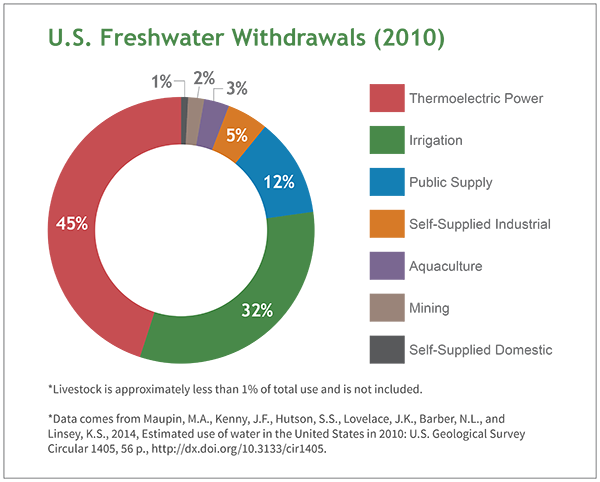
\includegraphics[width=8cm]{pie.png}
\end{wrapfigure}

This chart provided by the EPA below breaks down US freshwater withdrawals by use - showing that agriculture claims nearly one third of freshwater taken out of reservoirs in America\cite{us_epa_how_2017}. This, combined with public supply means that 44\% of US water withdrawal goes to farms or gardens, nearly 50\% of which, is wasted due to over-watering\cite{epa_watersense_nodate}. By conserving and intelligently applying the water used for irrigation at homes and farms, there exists the chance to reduce US freshwater withdrawal by nearly 22\%. This is water which by not removing from the its sources would work to protect from drought and changing ecosystems.\\

The system proposed above has plenty of commercial applications for homeowners, hobbyists, and even industrial farming. By keeping consumers informed about the environmental conditions in their gardens and by alleviating the necessarily workload and stress to maintain them, a modular garden monitoring system will work towards supporting green spaces and most importantly promoting sustainable habits and water conservation for the betterment of the world.

% Find reference chart of water waste in the Us
%Find a number for how much water we could prevent from being wasted
% find a reference that says over watered plants grow worse

\section*{Conclusion}

At a time when environmental awareness and sustainability efforts have never been more important, a tool to make sustainable gardening and landscaping more accessible for average homeowners is exactly what the world needs. The modular garden monitoring system proposed in this document, by providing helpful information for home gardeners and reducing the needed work to maintain a healthy garden, will support the creation of sustainable green spaces while conserving our very precious water supply.\newpage
% Keep it short – one to two sentences restating the need and urgency
\vspace{0.6cm}
\bibliography{bibliography}
\bibliographystyle{ieeetr}


\end{document}
